
%=========================================================
\section{Módulos del sistema}

    El sistema se encuentra organizado por módulos con la finalidad de agrupar y administrar de mejor manera los requerimientos funcionales del sistema. Dividir el sistema en módulos permite visualizar e identificar rápidamente aquellos aspectos funcionales que pueden tratarse conjuntamente. \\

    La figura \ref{fig:ModulosPAEAR} muestra los módulos propuestos de manera inicial para el \saear. Cada uno de estos módulos agrupan los casos de uso que poseen funcionalidad similar o que trabajan en conjunto para alcanzar un aspecto funcional del sistema. Cada uno de los módulos que se muestran en la figura se describen a continuación:

%    La figura \ref{fig:ModulosPAEAR} muestra los módulos que conforman el \saear. Cada uno de estos módulos agrupan los casos de uso que poseen funcionalidad similar o que trabajan en conjunto para alcanzar un aspecto funcional del sistema. Cada uno de los módulos que se muestran en la figura se describen a continuación:

    \begin{figure}[h!]
	\begin{center}
	      \fbox{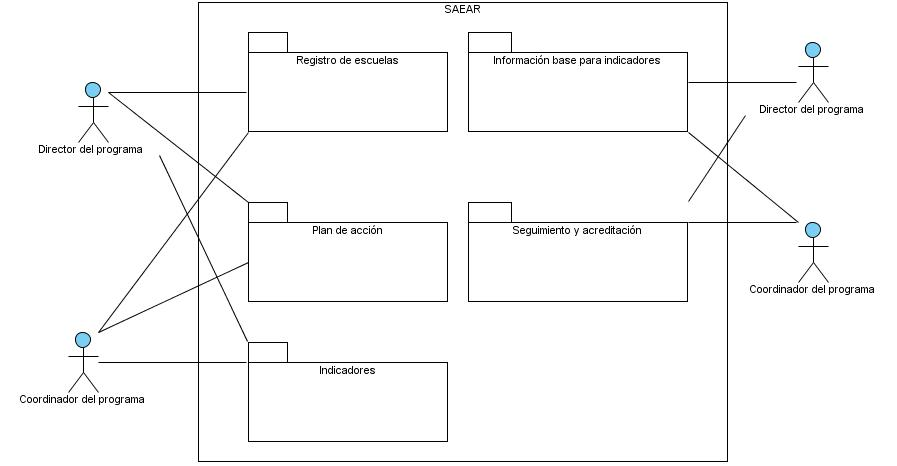
\includegraphics[width=\textwidth]{images/modulos.jpg}}
	\caption{Módulos del \saear.}
	\label{fig:ModulosPAEAR}
	\end{center}
    \end{figure}

    \begin{itemize}
	\item {\bf Registro de escuelas:} Agrupa los casos de uso que tienen que ver con el registro de la información de las escuelas y de su comité asociado. % así como los casos de uso que permiten a la SMAGEM la aprobación de la inscripción de las escuelas al programa.

	\item {\bf Información base para los indicadores:} Agrupa los casos de uso que proporcionan información ambiental base para los indicadores respecto a cada una de las líneas de acción. %También incluye los casos de uso que permiten a la SMAGEM la revisión, aprobación o rechazo de la información base para los indicadores.

	\item {\bf Plan de acción:} Agrupa los casos de uso que tienen que ver con la definición del plan de acción respecto a cada una de las líneas de acción por parte de las escuelas.% así como los casos de uso que permiten a la SMAGEM la revisión, aprobación o rechazo de un plan de acción ambiental.

	\item {\bf Seguimiento y Acreditación ambiental:} Contiene los casos de uso correspondientes al seguimiento de la ejecución del plan de acción de cada una de las escuelas registradas en el programa.%, así como de la acreditación de las mismas de acuerdo al informe final de actividades revisado por SMAGEM.

	\item {\bf indicadores:} Integra los casos de uso referentes a los indicadores ambientales y de sustentabilidad de la escuela.

%	\item {\bf Administración de usuarios:} Integra los casos de uso referentes a la administración de los usuarios y al control de acceso al sistema.

	%El presente documento expone en detalle la información correspondiente al módulo de \textbf{Registro de escuelas}.

    \end{itemize}

%=========================================================
\section{Actores del sistema}\label{sec:Comportamiento:ActoresSistema}

Los actores son los perfiles asociados a las diversas áreas y/u organizaciones que intervienen en el proceso. Se han identificado los actores de acuerdo a las actividades y responsabilidades dentro del \paear, los cuales se muestran en la figura \ref{fig:perfilesPAEAR} y se describen a continuación.

%    Los actores son los perfiles asociados a las diversas áreas y/u organizaciones que intervienen en el proceso. Se han identificado los actores de acuerdo a las actividades y responsabilidades dentro del \paear respecto al módulo de \textbf{Registro de escuelas}, los cuales se muestran en la figura \ref{fig:perfilesPAEAR} y se describen a continuación. 
    %y responsabilidades dentro del \paear - \saear, los cuales se describen a continuación.

    \begin{figure}[h!]
      \begin{center}
	  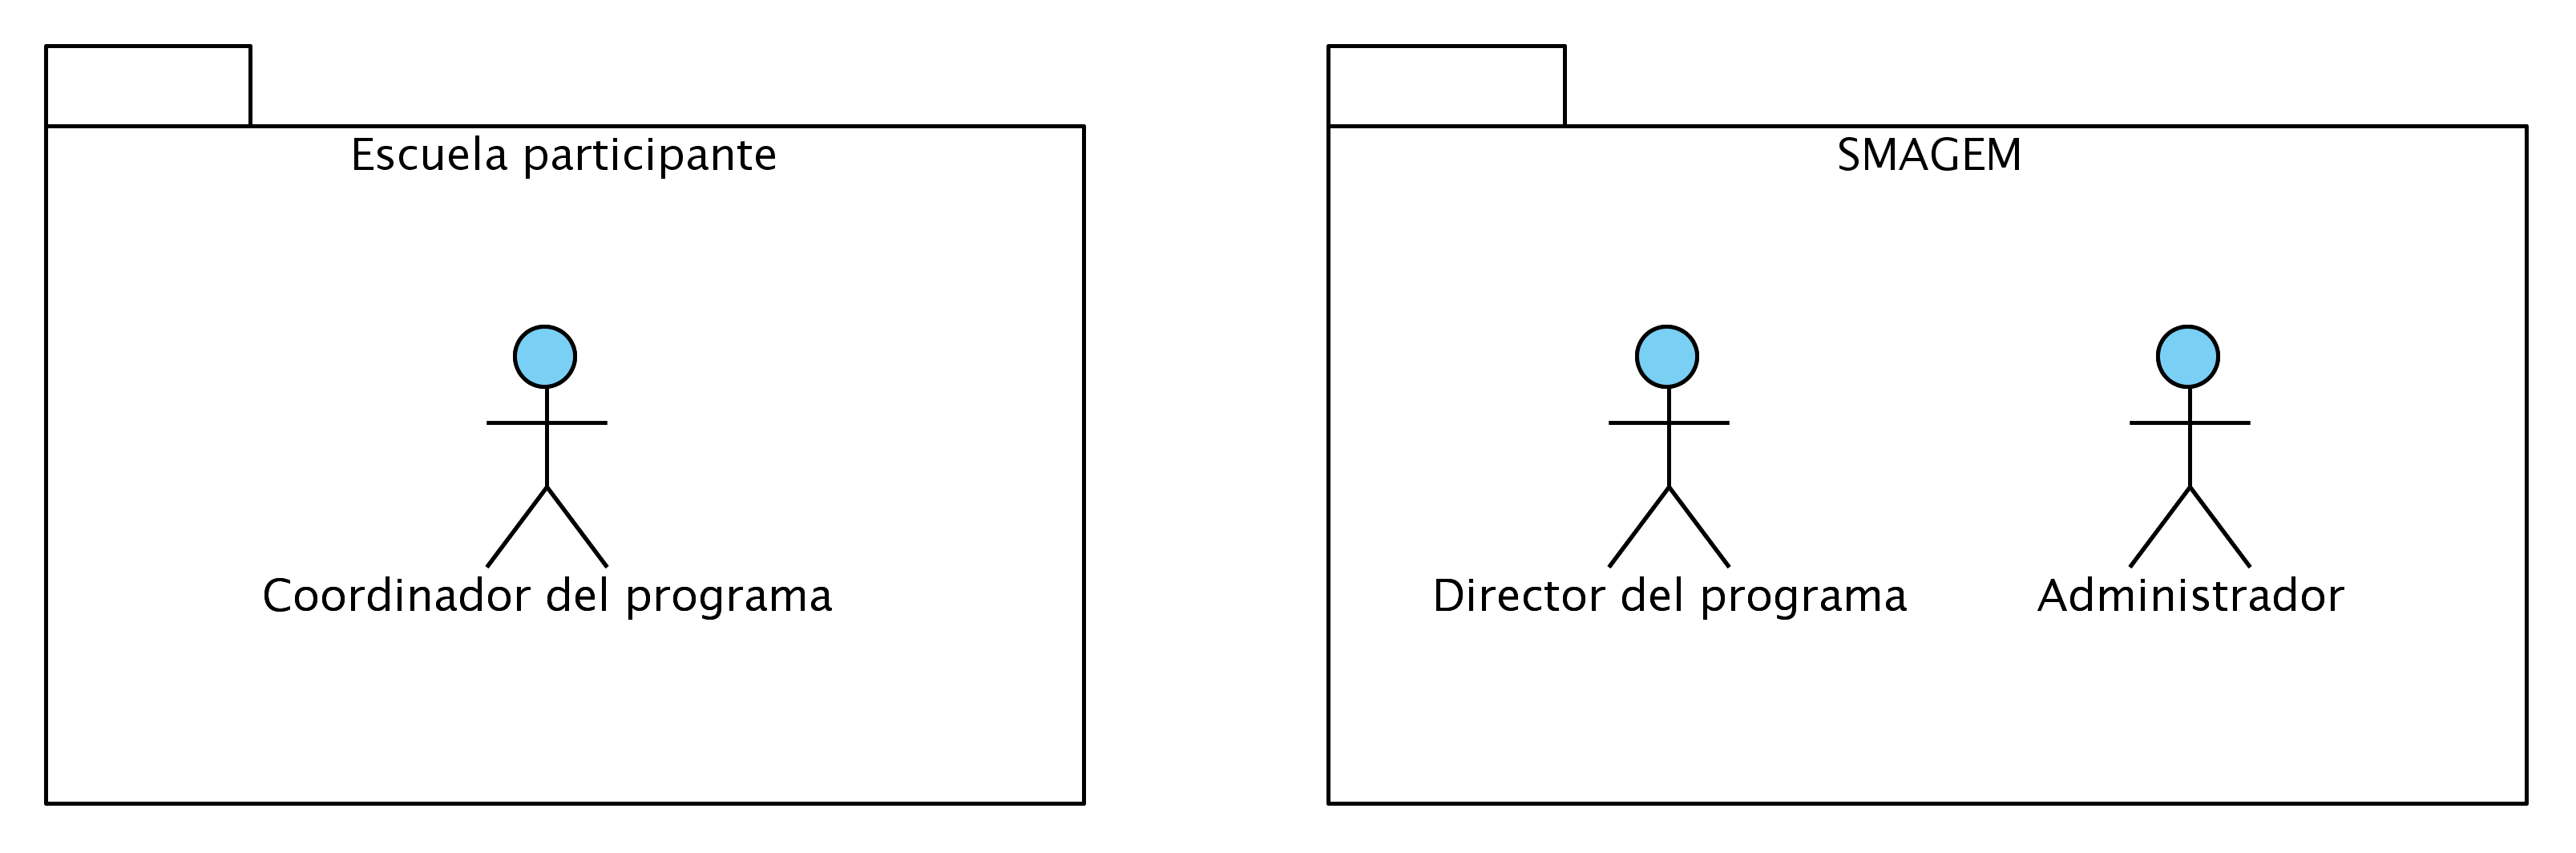
\includegraphics[width=0.6\textwidth]{images/actores/Actores.png}
      \caption{Perfiles identificados.}
      \label{fig:perfilesPAEAR}
      \end{center}
    \end{figure}

%--------------------------------------------------------------------------------------------------
    \begin{actor}{Coordinador del programa}{usuarioEscuela}{Persona designada por la escuela para operar todo lo referente a la participación de la escuela y de su comité en el PAEAR.}

	\item[Área:] Escuela participante.

	\item[Responsabilidades:] \hspace{1pt}
	
		\begin{itemize}

		    %%%%%%%%%%%% REGISTRO %%%%%%%%%%%%
		    %Escuela
		    \item Solicitar la inscripción de su escuela en el programa.
		    \item Registrar y modificar la información de su escuela en el programa durante el periodo de registro.
		    %Coordinador del programa
		    \item Registrar al coordinador y al responsable del programa dentro del periodo de registro.
		    % Responsable del programa
		    \item Modificar la información del responsable del programa dentro del periodo de registro.	
		    %Integrantes de las líneas de acción
		    \item Registrar o dar de baja a los integrantes de las líneas de acción dentro del periodo de registro.
		    \item Modificar la información de los integrantes de las líneas de acción dentro del periodo de registro.
		    %General: información escolar, coordinador, responsable e integrantes de líneas de acción
		    \item Visualizar la información de registro de su escuela y de los miembros del comité asociado.

		    %%%%%%%%%%%% DIAGNÓSTICO %%%%%%%%%%%%
		    %Descargar fotmatos y cuestionarios			
		    %\item Descargar los formatos y cuestionarios de diagnóstico dentro del periodo asignado.
		    %Registro formatos y cuestionarios
%			\item Registrar la información correspondiente a los formatos y cuestionarios de diagnóstico dentro del periodo asignado.
		    %Modificación formatos y cuestionarios
%			\item Modificar la información registrada en los formatos y cuestionarios de diagnóstico dentro del periodo asignado.
		    %Envío de diagnóstico
%			\item Enviar su diagnóstico para su aprobación.

			%%%%%%%%%%%% INFORMACIÓN BASE PARA INDICADORES %%%%%%%%%%%%
			\item Registrar y modificar la información base para indicadores de agua dentro del periodo de registro de información base.
			\item Registrar y modificar la información base para indicadores de residuos sólidos dentro del periodo de registro de información base.
			\item Registrar y modificar la información base para indicadores de energía dentro del periodo de registro de información base.
			\item Registrar y modificar la información base para indicadores de biodiversidad dentro del periodo de registro de información base.
			\item Registrar y modificar la información base para indicadores de ambiente escolar dentro del periodo de registro de información base.
			\item Registrar y modificar la información base para indicadores de consumo responsable	dentro del periodo de registro de información base.

			
		    %%%%%%%%%%%% PLAN DE ACCIÓN %%%%%%%%%%%%
			\item Registrar, modificar y eliminar los objetivos asociados a las líneas de acción dentro del periodo de registro del plan de acción.
			\item Registrar, modificar y eliminar las metas asociadas a cada línea de acción dentro del periodo de registro del plan de acción.
			\item Registrar, modificar y eliminar las acciones asociadas a las metas de cada línea de acción dentro del periodo de registro del plan de acción.

		    %%%%%%%% SEGUIMIENTO Y ACREDITACIÓN %%%%%%%%
			\item Registrar, modificar y eliminar el avance de las metas asociadas a cada línea de acción dentro del periodo de registro de informe de avance.
			\item Registrar, modificar y eliminar las acciones asociadas a las metas de cada línea de acción  dentro del periodo de registro de informe de avance.
			\item Actualizar la información para el cálculo de los indicadores.

			\item Enviar la información base para indicadores, el plan de acción y los informes de avances del plan de acción para su revisión por parte de SMAGEM.
			\item Consultar los indicadores ambientales y de sustentabilidad.
		\end{itemize}


	\item[Perfil:] \hspace{1pt}
		\begin{itemize}
		    \item Conocer el objetivo del PAEAR.
		    \item Conocimientos básicos en materia ambiental.
		    \item Conocimientos en el uso de computadora.
		    \item Contar con una cuenta de correo electrónico.
	    \end{itemize}

	\item[Cantidad:] Uno por escuela participante.

\end{actor}

%--------------------------------------------------------------------------------------------------
\begin{actor}{Director del programa}{usuarioSMAGEM}{Director del programa de Acreditación de Escuelas Ambientalmente Responsables en SMAGEM.}

    \item[Área:] SMAGEM.
    \item[Responsabilidades:] \hspace{1pt}

	\begin{itemize}
	      %%%%%%%% REGISTRO %%%%%%%%
	      \item Visualizar la información de las escuelas que solicitan su inscripción al programa.
	      \item Aceptar o rechazar la solicitud de inscripción de las escuelas en el programa.
	      %%%%%%%% DIAGNÓSTICO %%%%%%%%
%			\item Visualizar la información de las escuelas que solicitan su aprobación de diagnóstico ambiental.
%			\item Aceptar o rechazar la solicitud de aprobación de diagnóstico ambiental.

	      %%%%%%%% INFORMACIÓN BASE PARA INDICADORES %%%%%%%%
		  \item Visualizar la información de las escuelas que enviaron su información base para indicadores.
		  \item Aceptar o rechazar la solicitud de aprobación de la información base para indicaadores.
%			\item Visualizar la información de las escuelas que solicitan su aprobación de plan de acción ambiental.
%			\item Aceptar o rechazar la solicitud de aprobación de plan de acción ambiental.

	      %%%%%%%% PLAN DE ACCIÓN %%%%%%%%
		  \item Visualizar la información de las escuelas que enviaron su plan de acción.
		  \item Aceptar o rechazar la solicitud de aprobación del plan de acción.
		  
		  %%%%%%%% SEGUIMIENTO Y ACREDITACIÓN %%%%%%%%%
		  \item Visualizar la información de las escuelas que enviaron su informe de avance de plan de acción.
		  \item Aceptar o rechazar la solicitud de aprobación del avance del plan de acción.
		  \item Aceptar o rechazar la acreditación de la escuela.
		  
		  %%%%%%%%% INDICADORES %%%%%%%%%%%%%
		  \item Consultar los indicadores de eficacia y eficiencia del programa.
		  \item Consultar los indicadores de educación ambiental.
		  \item Consultar los indicadores ambientales y de sustentabilidad.		  
    \end{itemize}

    \item[Perfil:] \hspace{1pt}

	\begin{itemize}

	    \item Conocimientos sobre la operación del sistema.
	    \item Contar con un amplio conocimiento sobre el PAEAR.
	    \item Conocimientos en el uso de computadora.
	    \item Contar con una cuenta de correo electrónico.

	\end{itemize}

    \item[Cantidad:] Uno para la SMAGEM.

\end{actor}

%--------------------------------------------------------------------------------------------------
%\begin{actor}{Administrador}{administrador}{Persona encargada de administrar y dar soporte técnico al sistema.}
%
%    \item[Área:] SMAGEM.
%
%    \item[Responsabilidades:] \hspace{1pt}
%
%	\begin{itemize}
%
%	  \item Dar soporte técnico al sistema en lo referente a conectividad y acceso por parte de los usuarios.
%    %\item Puede realizar todas las operaciones de los demás usuarios por instrucciones del Director del Programa.
%
%	\end{itemize}
%
%    \item[Perfil:] \hspace{1pt}
%
%      \begin{itemize}
%
%	\item Conocimientos técnicos y de operación del sistema.
%	\item Conocimientos del sistema operativo sobre el cual se instale el sistema.
%	\item Conocimientos acerca de la administración de sistemas.
%	\item Contar con una cuenta de correo electrónico.
%
%      \end{itemize}
%
%    \item[Cantidad:] Uno para la SMAGEM.
%
%\end{actor}


%====================================================================================
\section{Casos de Uso del módulo de Registro de Escuelas}

    La figura \ref{fig:casosUso:registro} muestra los casos de uso que integran la funcionalidad del módulo de Registro de escuelas, que se refieren al registro, modificación y visualización de la información escolar y del comité asociado a cada escuela.

    \begin{figure}[h!]
	\begin{center}
	    \fbox{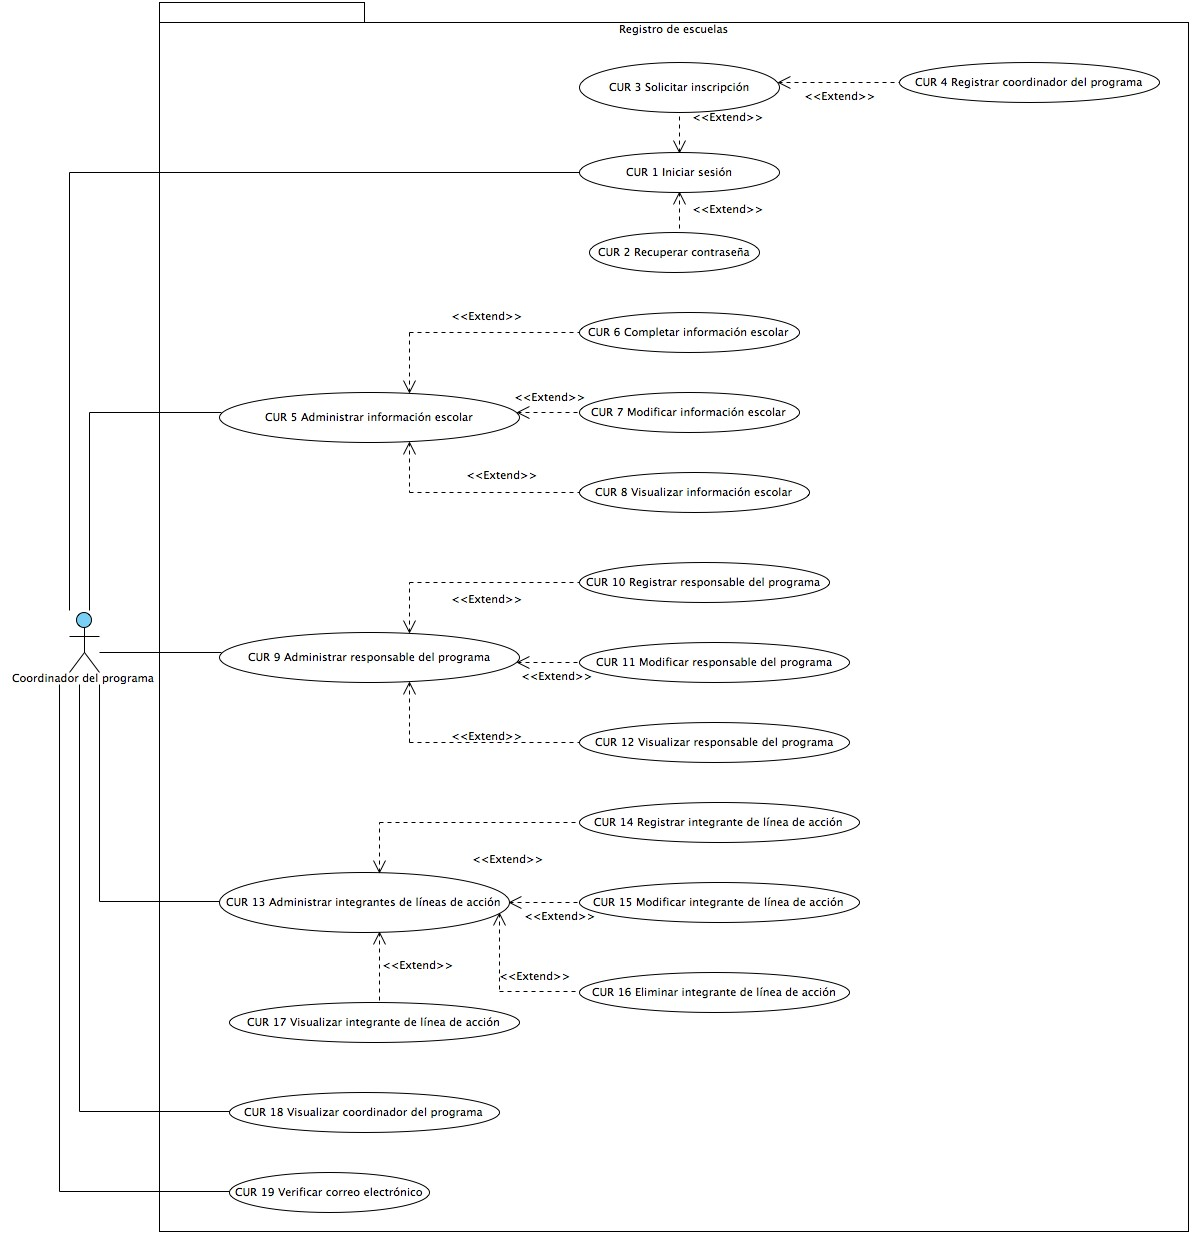
\includegraphics[width=.9\textwidth]{images/CasosUso/Registro.png}}
	\caption{Diagrama de casos de uso para el módulo de Registro de escuelas. \label{fig:casosUso:registro}}
	\end{center}
    \end{figure}

\section{Casos de Uso del módulo de Información base para indicadores}
La figura \ref{fig:casosUso:comite} muestra los casos de uso que integran la funcionalidad necesaria para la obtención de la información base para los indicadores ambientales y de sustenteabilidad de la escuela y que se refieren al registro y modificación de su información.

 \begin{figure}[h!]
     \begin{center}
         \fbox{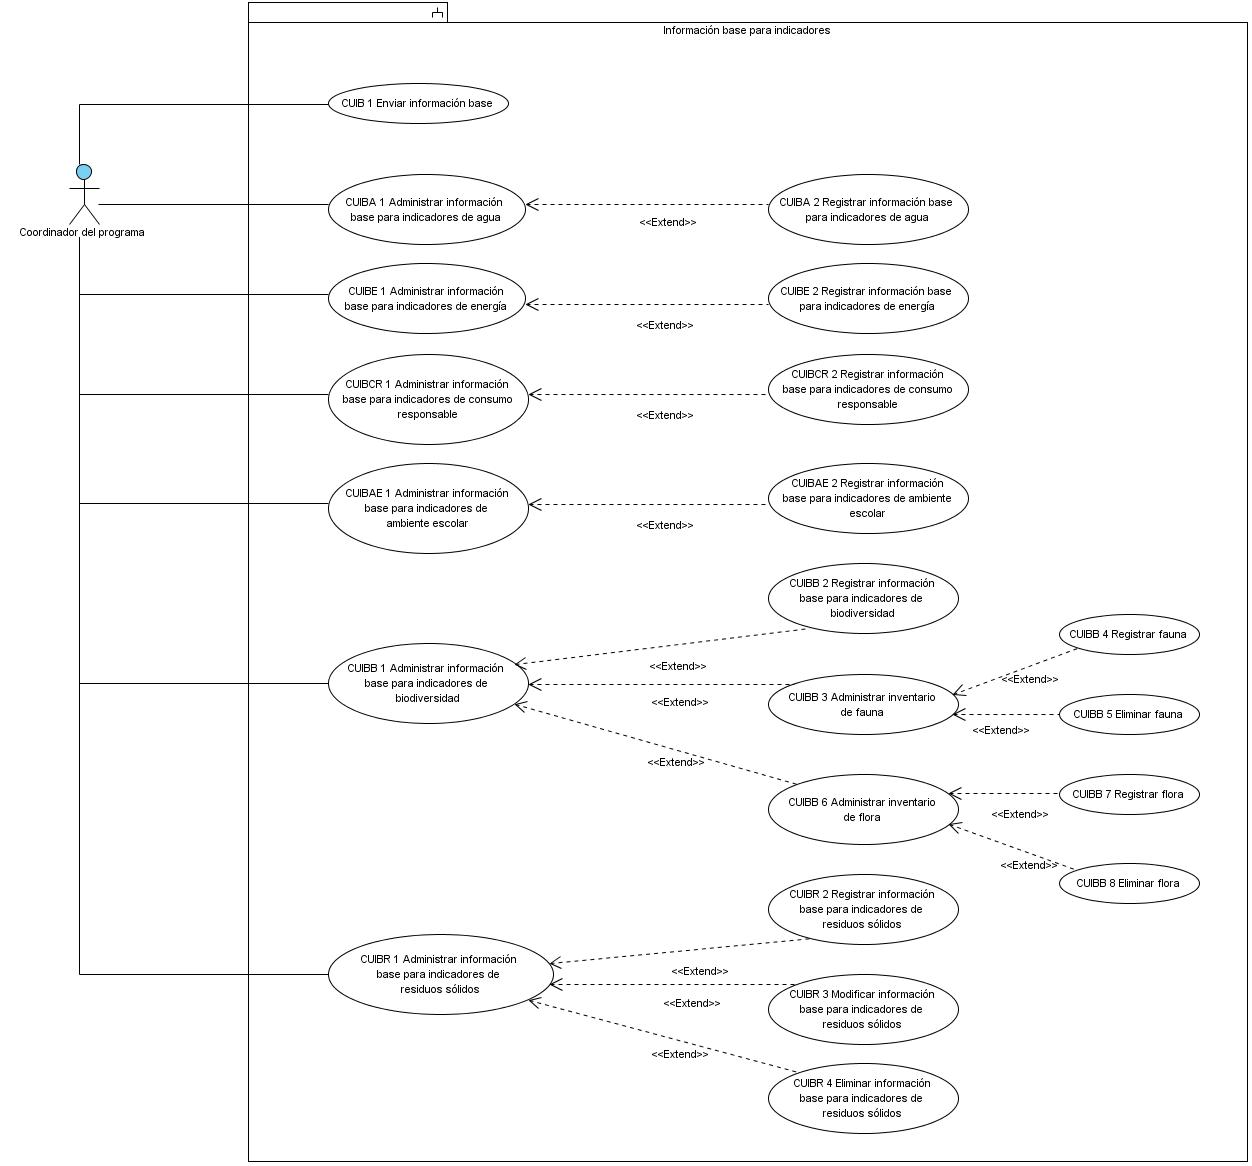
\includegraphics[angle=90, height=0.9\textheight]{images/CasosUso/informacionBase.jpg}}
     \caption{Diagrama de casos de uso para el módulo de Información base para indicadores.}
     \label{fig:casosUso:comite}
     \end{center}
 \end{figure}

\section{Casos de Uso del módulo de Plan de acción}
La figura \ref{fig:casosUso:plan} muestra los casos de uso que integran la funcionalidad del módulo de Plan de acción, los cuales permiten el registro y modificación del plan de acción de la escuela. 

\begin{figure}[h!]
    \begin{center}
        \fbox{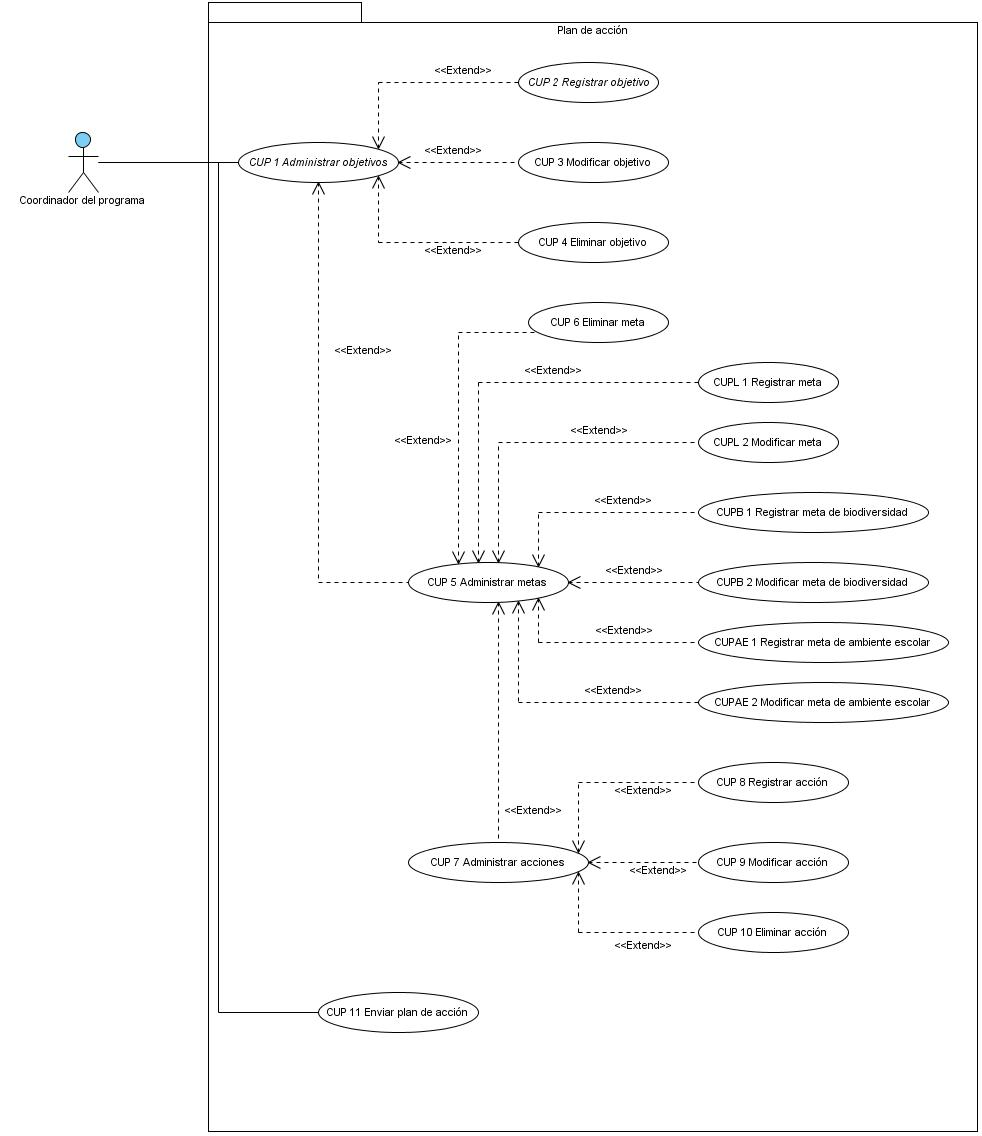
\includegraphics[width=\textwidth]{images/CasosUso/plan.jpg}}
    \caption{Diagrama de casos de uso para el módulo de Plan de acción.}
    \label{fig:casosUso:plan}
    \end{center}
\end{figure}

\section{Casos de Uso del módulo de Seguimiento y acreditación}
La figura \ref{fig:casosUso:seguimiento} muestra los casos de uso que integran la funcionalidad del módulo de Seguimiento y acreditación, los cuales permiten el registro y modificación de los avances realizados en el plan de acción de la escuela. 

\begin{figure}[h!]
    \begin{center}
        \fbox{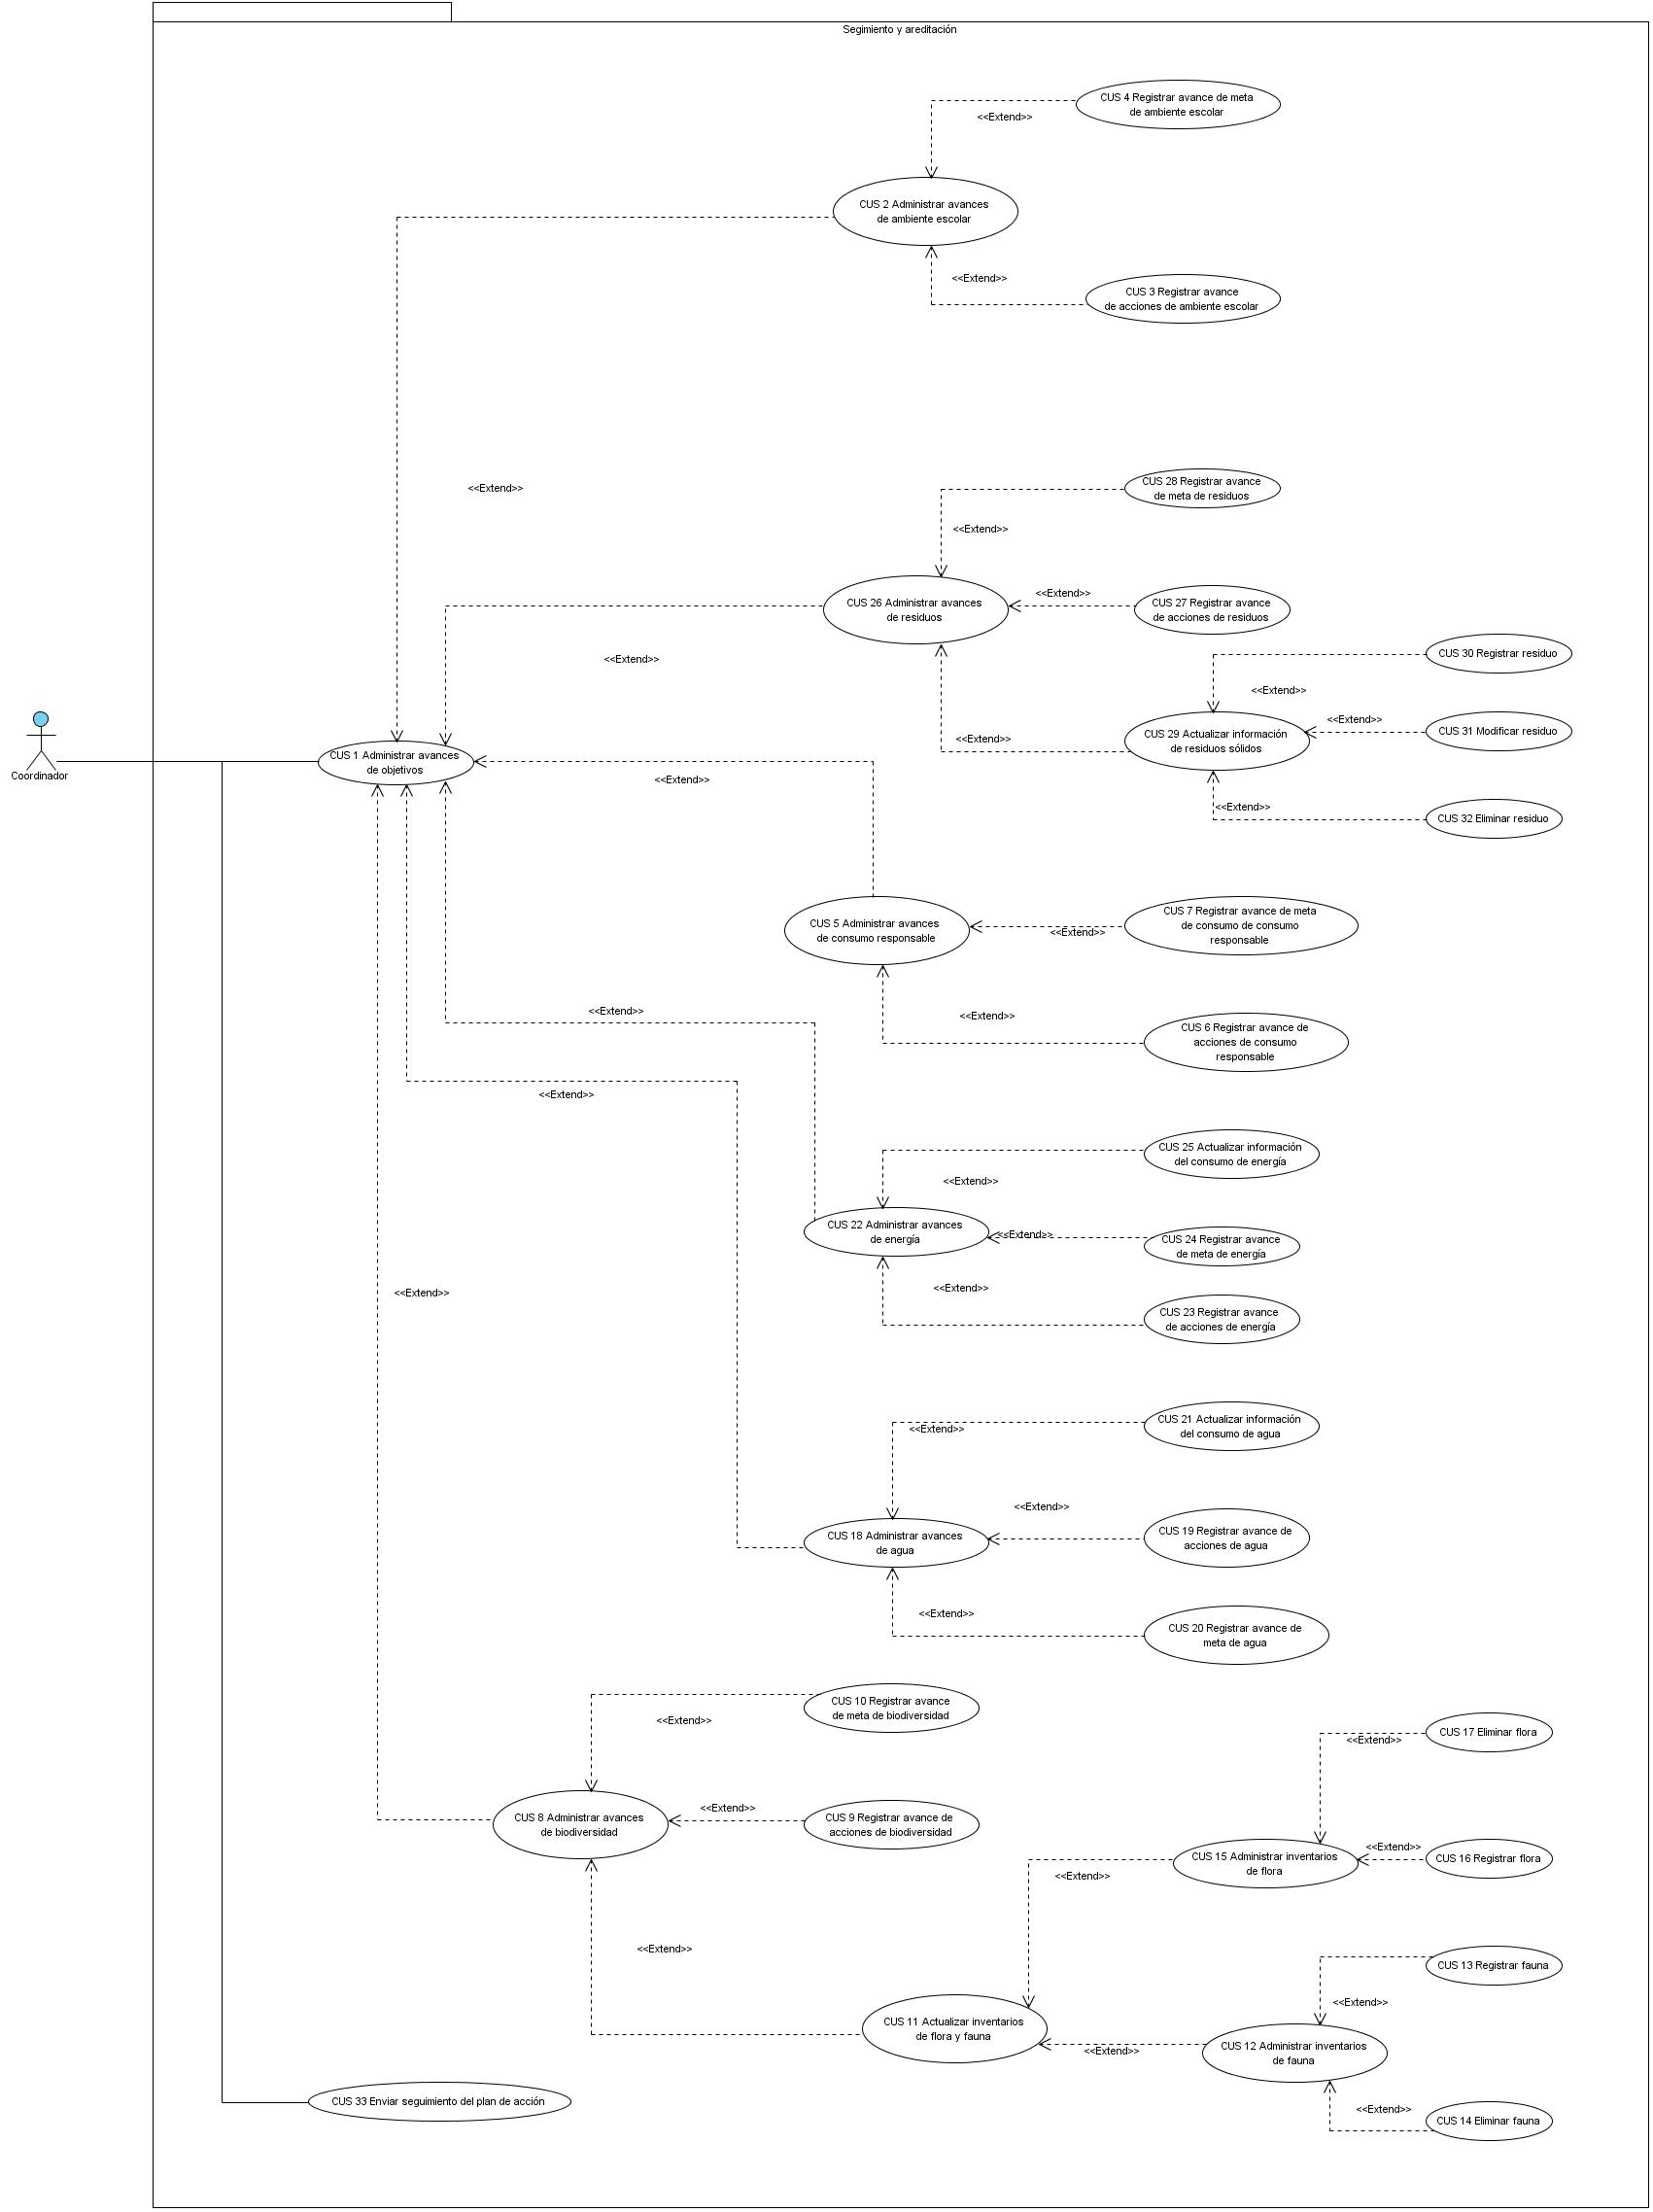
\includegraphics[width=\textwidth]{images/CasosUso/Seguimiento.jpg}}
    \caption{Diagrama de casos de uso para el módulo de Seguimiento y acreditación.}
    \label{fig:casosUso:seguimiento}
    \end{center}
\end{figure}

\section{Casos de Uso del módulo de Indicadores}
La figura \ref{fig:casosUso:indicadores} muestra los casos de uso que integran la funcionalidad del módulo de Indicadores, los cuales permiten la visualización de los resultado obtenidos en los indicadores ambientales y de sustententabilidad de la escuela. 

\begin{figure}[h!]
    \begin{center}
        \fbox{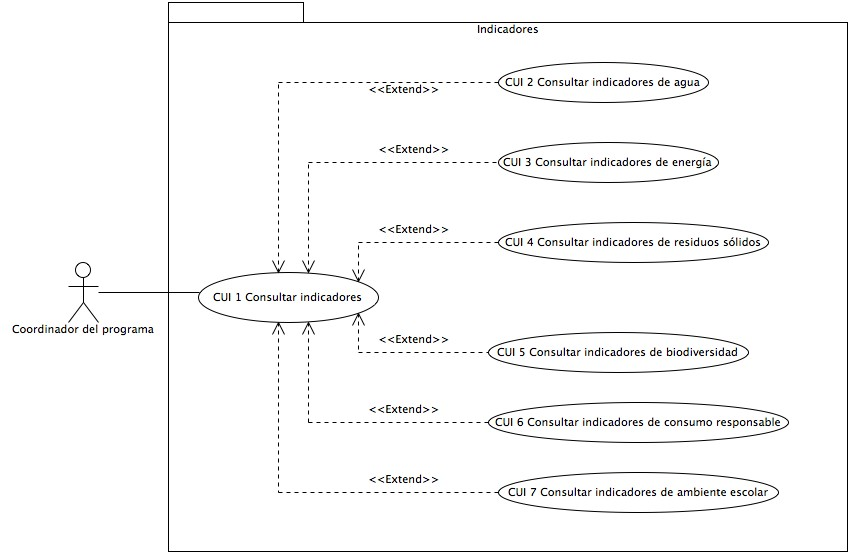
\includegraphics[width=\textwidth]{images/CasosUso/Indicadores.png}}
    \caption{Diagrama de casos de uso para el módulo de Indicadores.}
    \label{fig:casosUso:indicadores}
    \end{center}
\end{figure}